\documentclass[11pt]{article}
\usepackage[a4paper,margin=1in]{geometry}
\usepackage{amsmath,amssymb,amsthm,mathtools}
\usepackage{graphicx}
\usepackage[hidelinks]{hyperref}
\emergencystretch=3em

\newtheorem{theorem}{Theorem}
\newtheorem{lemma}[theorem]{Lemma}
\newcommand{\Ht}[2]{\widetilde H^{#1,#2}}
\makeatletter
\renewcommand{\@seccntformat}[1]{\csname the#1\endcsname\hspace{0.75em}}
\makeatother

\title{A Boundary-Trace Counterexample to the\\
Power Law for Optimal Fractional Poincar\'e Constants}
\author{A full counterexample to Conjecture 5.8 of arXiv:2203.02425}
\date{August 11, 2026}

\begin{document}
\maketitle

\begin{abstract}
Railo and Zimmermann conjecture that every optimal fractional Poincar\'e
constant is a power of any one such constant.  We disprove this already for
$p=2$ on the interval $(0,\pi)$.  The optimal order-one constant is
$C_{1,0}=1$, attained by the zero extension of $\sin x$.  At order two, the
space of zero extensions has the additional clamped trace $u'=0$ at both
endpoints.  Compactness and the equality case of the sharp Poincar\'e inequality
then give $C_{2,0}<1$.  Thus $C_{2,0}\ne C_{1,0}^2$.
\end{abstract}

\noindent\textbf{Status.}
\texttt{full counterexample; likely valid}.  Human review is recommended.

\section{The conjecture}

For an open set $\Omega\subset\mathbb R^n$, the source uses
\[
 \Ht{r}{p}(\Omega)=
 \overline{C_c^\infty(\Omega)}^{\,H^{r,p}(\mathbb R^n)}.
\]
For $p=2$, write $C_{r,z}(\Omega)$ for the optimal constant in
\begin{equation}\label{eq:def}
 \|(-\Delta)^{z/2}u\|_{L^2(\mathbb R^n)}
 \le C_{r,z}(\Omega)
 \|(-\Delta)^{r/2}u\|_{L^2(\mathbb R^n)},
 \qquad u\in\widetilde H^r(\Omega).
\end{equation}
Conjecture 5.8 asserts that, whenever $r>z\ge0$ and $t>s\ge0$,
\begin{equation}\label{eq:conj}
 C_{t,s}(\Omega)=C_{r,z}(\Omega)^{(t-s)/(r-z)}.
\end{equation}

\begin{center}
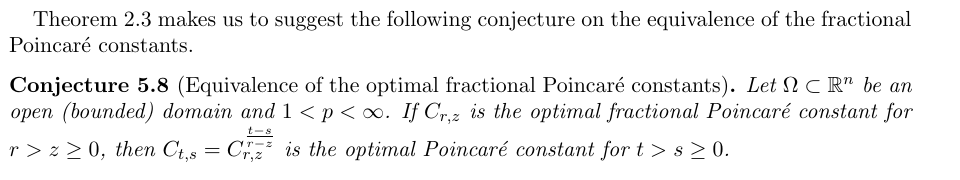
\includegraphics[width=.96\linewidth]{figures/conjecture_crop.png}
\end{center}

\section{The interval and its traces}

Take
\[
 n=1,\qquad p=2,\qquad \Omega=(0,\pi).
\]
Functions are identified with their zero extensions to $\mathbb R$.
Standard one-dimensional trace theory gives
\begin{align*}
 \widetilde H^1(0,\pi)&=H_0^1(0,\pi),\\
 \widetilde H^2(0,\pi)&=H_0^2(0,\pi)
 =\{u\in H^2(0,\pi):u(0)=u(\pi)=u'(0)=u'(\pi)=0\},
\end{align*}
where the equalities mean zero extension into the corresponding space on
$\mathbb R$.  Plancherel gives
\begin{equation}\label{eq:plancherel}
 \|(-\Delta)^{1/2}u\|_2=\|u'\|_2,
 \qquad
 \|(-\Delta)u\|_2=\|u''\|_2
\end{equation}
on these spaces.

The extra order-two trace is the decisive point: the zero extension of
$\sin x$ belongs to $\widetilde H^1(0,\pi)$ but not to
$\widetilde H^2(0,\pi)$.

\section{The order-one optimum}

The sharp Dirichlet Poincar\'e inequality on $(0,\pi)$ is
\[
 \|u\|_2\le\|u'\|_2\qquad(u\in H_0^1(0,\pi)),
\]
with equality exactly for scalar multiples of $\sin x$.  The zero extension of
$\sin x$ is an admissible element of $\widetilde H^1(0,\pi)$.  Consequently,
\begin{equation}\label{eq:c10}
 C_{1,0}(0,\pi)=1.
\end{equation}

\section{Strict loss at order two}

For $u\in\widetilde H^2(0,\pi)$, the Dirichlet inequality and the mean-zero
Wirtinger inequality applied to $u'$ give
\begin{equation}\label{eq:chain}
 \|u\|_2\le\|u'\|_2\le\|u''\|_2.
\end{equation}
Indeed, $u$ has zero endpoint values and
$\int_0^\pi u'(x)\,dx=u(\pi)-u(0)=0$.  Thus
$C_{2,0}(0,\pi)\le1$.

We need strictness, because the conjecture concerns the optimal constant.  The
supremum
\[
 C_{2,0}(0,\pi)=
 \sup_{0\ne u\in\widetilde H^2(0,\pi)}
 \frac{\|u\|_2}{\|u''\|_2}
\]
is attained.  To see this, normalize a maximizing sequence by
$\|u_j''\|_2=1$.  The two inequalities in \eqref{eq:chain} bound it in $H^2$.
A weakly convergent subsequence converges strongly in $L^2$ by Rellich
compactness, and the closed trace conditions persist.  Weak lower
semicontinuity, followed by a rescaling if necessary, yields a maximizer.

Suppose now that $C_{2,0}(0,\pi)=1$, and let $u$ be a nonzero maximizer.
Then equality holds throughout \eqref{eq:chain}.  Equality in the first,
sharp Dirichlet inequality forces
\[
 u(x)=A\sin x.
\]
But $u\in\widetilde H^2(0,\pi)$ also has $u'(0)=0$, so $A=0$, a
contradiction.  Hence
\begin{equation}\label{eq:c20}
 C_{2,0}(0,\pi)<1.
\end{equation}

\begin{theorem}
Conjecture 5.8 is false.  For $\Omega=(0,\pi)$ and $p=2$,
\[
 C_{2,0}(\Omega)<1=C_{1,0}(\Omega)^2,
\]
whereas \eqref{eq:conj} with $(r,z,t,s)=(1,0,2,0)$ predicts equality.
\end{theorem}

\section{Mechanism, verification, and novelty}

The conjectured interpolation value remains a valid upper bound; it simply need
not be optimal.  The obstruction is the changing optimization domain.  Raising
the zero-extension Sobolev order from one to two imposes the additional normal
trace $u'=0$, excluding the order-one extremizer.  After rescaling, the same
argument gives a counterexample on every bounded interval.

For orientation only, the order-two extremizer is the first clamped-beam mode:
$C_{2,0}(0,\pi)=\pi^2/\beta_1^2\approx0.441$, where $\beta_1\approx4.730$ is
the first positive root of $\cos\beta\cosh\beta=1$.  This numerical
identification is not used in the proof; the accompanying script checks it.

The 2023 journal version retains Conjecture 5.8.  A bounded search using its
exact title and wording, the arXiv identifier, and later papers citing the
source found no resolution or matching interval counterexample.  Independent
mathematical and literature review is nevertheless recommended.

\begin{thebibliography}{9}
\bibitem{RZ}
J. Railo and P. Zimmermann,
\emph{Fractional Calder\'on problems and Poincar\'e inequalities on unbounded
domains}, J. Spectr. Theory 13 (2023), 63--131, Conjecture 5.8.
\url{https://doi.org/10.4171/JST/444}
\end{thebibliography}

\end{document}
